%%%%%%%%%%%%%%%%%%%%%%%%%%%%%%%%%%%%%%%%%
% University Assignment Title Page 
% LaTeX Template
% Version 1.0 (27/12/12)
%
% This template has been downloaded from:
% http://www.LaTeXTemplates.com
%
% Original author:
% WikiBooks (http://en.wikibooks.org/wiki/LaTeX/Title_Creation)
%
% License:
% CC BY-NC-SA 3.0 (http://creativecommons.org/licenses/by-nc-sa/3.0/)
% 
% Instructions for using this template:
% This title page is capable of being compiled as is. This is not useful for 
% including it in another document. To do this, you have two options: 
%
% 1) Copy/paste everything between \begin{document} and \end{document} 
% starting at \begin{titlepage} and paste this into another LaTeX file where you 
% want your title page.
% OR
% 2) Remove everything outside the \begin{titlepage} and \end{titlepage} and 
% move this file to the same directory as the LaTeX file you wish to add it to. 
% Then add \input{./title_page_1.tex} to your LaTeX file where you want your
% title page.
%
%%%%%%%%%%%%%%%%%%%%%%%%%%%%%%%%%%%%%%%%%
%\title{Title page with logo}
%----------------------------------------------------------------------------------------
%	PACKAGES AND OTHER DOCUMENT CONFIGURATIONS
%----------------------------------------------------------------------------------------

\documentclass[12pt]{article}
\usepackage[english]{babel}
\usepackage[utf8x]{inputenc}
\usepackage{amsmath}
\usepackage{graphicx}
\usepackage{hyperref}
\usepackage{enumitem}

\usepackage[colorinlistoftodos]{todonotes}

\begin{document}

\begin{titlepage}

\newcommand{\HRule}{\rule{\linewidth}{0.5mm}} % Defines a new command for the horizontal lines, change thickness here

\center % Center everything on the page
 
%----------------------------------------------------------------------------------------
%	HEADING SECTIONS
%----------------------------------------------------------------------------------------

\textsc{\LARGE Università degli studi di Milano-Bicocca}\\[1cm] % Name of your university/college
\textsc{\Large Advanced Machine Learning }\\[0.3cm] % Major heading such as course name
\textsc{\large Final Project}\\[0.1cm] % Minor heading such as course title

%----------------------------------------------------------------------------------------
%	TITLE SECTION
%----------------------------------------------------------------------------------------

\HRule \\[0.4cm]
{ \huge \bfseries Electical Motor Something Something}\\[0.2cm] % Title of your document
\HRule \\[1.5cm]
 
%----------------------------------------------------------------------------------------
%	AUTHOR SECTION
%----------------------------------------------------------------------------------------

\large
\emph{Authors:}\\
Federico Moiraghi - xxxxxx - f.xx@@campus.unimib.it\\
Pranav Kasela - 846965 - p.kasela@campus.unimib.it \\   % Your name
Roberto Berlucchi - xxxxxx - r.xx@@campus.unimib.it   \\[0.5cm] % Your name

% If you don't want a supervisor, uncomment the two lines below and remove the section above
%\Large \emph{Author:}\\
%John \textsc{Smith}\\[3cm] % Your name

%----------------------------------------------------------------------------------------
%	DATE SECTION
%----------------------------------------------------------------------------------------

{\large 2019-2020}\\[1cm] % Date, change the \today to a set date if you want to be precise

%----------------------------------------------------------------------------------------
%	LOGO SECTION
%----------------------------------------------------------------------------------------


\includegraphics{imgs/logo.png}\\[1cm] % Include a department/university logo - this will require the graphicx package
 
%----------------------------------------------------------------------------------------

\vfill % Fill the rest of the page with whitespace

\end{titlepage}


\begin{abstract}
The ABSTRACT is not a part of the body of the report itself. Rather, the abstract is a brief summary of the report contents that is often separately circulated so potential readers can decide whether to read the report. The abstract should very concisely summarize the whole report: why it was written, what was discovered or developed, and what is claimed to be the significance of the effort. The abstract does not include figures or tables, and only the most significant numerical values or results should be given.
\end{abstract}

\section{Introduction}
The data set comprises several sensor data collected from a permanent magnet synchronous motor (PMSM) deployed on a test bench. 
The PMSM represents a German OEM's prototype model. 
Test bench measurements were collected by the LEA department at Paderborn University.

The recordings are sampled at a frequency of 2 Hz and is divided in various profiles and has a total of $998070$ observations. 
Each profile indicates a different session and each session can have different length varying from one to six hours.\\
The input variables are:
\begin{itemize}[topsep=0ex, noitemsep]
    \item \textbf{Ambient temperature} as measured by a thermal sensor located closely to the stator;
    \item \textbf{Coolant temperature}, the motor is water cooled and the measurement is taken at outflow;
    \item The current and voltage are transformed through a $dq0$ transformation in a d-q coordinate system, it basically converts a three phase balanced reference system (in an AC system) into 2 coordinates, denoted by d and q, via a rotating reference frame with angle $\theta$.
    The currents are denoted by \textbf{i\_d} and \textbf{i\_q} and the voltages are denoted by \textbf{u\_d} and \textbf{u\_q};
    \item \textbf{Motor speed}.
\end{itemize}
The target variables are:
\begin{itemize}[topsep=0ex, noitemsep]
    \item \textbf{pm}: Permanent Magnet surface temperature representing the rotor temperature, measured with an infrared thermography unit.
    \item \textbf{stator\_yoke}, \textbf{stator\_tooth}, \textbf{stator\_winding} respectively stator yoke, tooth and winding temperature measured with a thermal sensor.
\end{itemize}
In some of the variables some random walks are introduced to simulate real world driving cycles.\\
The main obective is to create a lightweight model to predict the pm and stator variables minimizing the MSE because the model needs to be deployed using the model with best cost-precision ratio, a secondary objective is to predict more accurately higher temperature than the lower temperature using a modified loss.

\section{Datasets}
The data set can be found on Kaggle on the following link\footnote{\href{https://www.kaggle.com/wkirgsn/electric-motor-temperature}{https://www.kaggle.com/wkirgsn/electric-motor-temperature}}.
From the data set the torque is immediately excluded, this particular variable is considered unreliable from the data set provider itself.

The data set is divided into train-validation-test, the validation data consists of profile\_id included in $20,31,46,54, 62, 70, 79, 72$, the test set in $35, 42$ and the training set consists of all the other profiles. Their relative distributions are plotting in the Figure \ref{fig:dist_plot}.
\begin{figure}[!h]
    \centering
    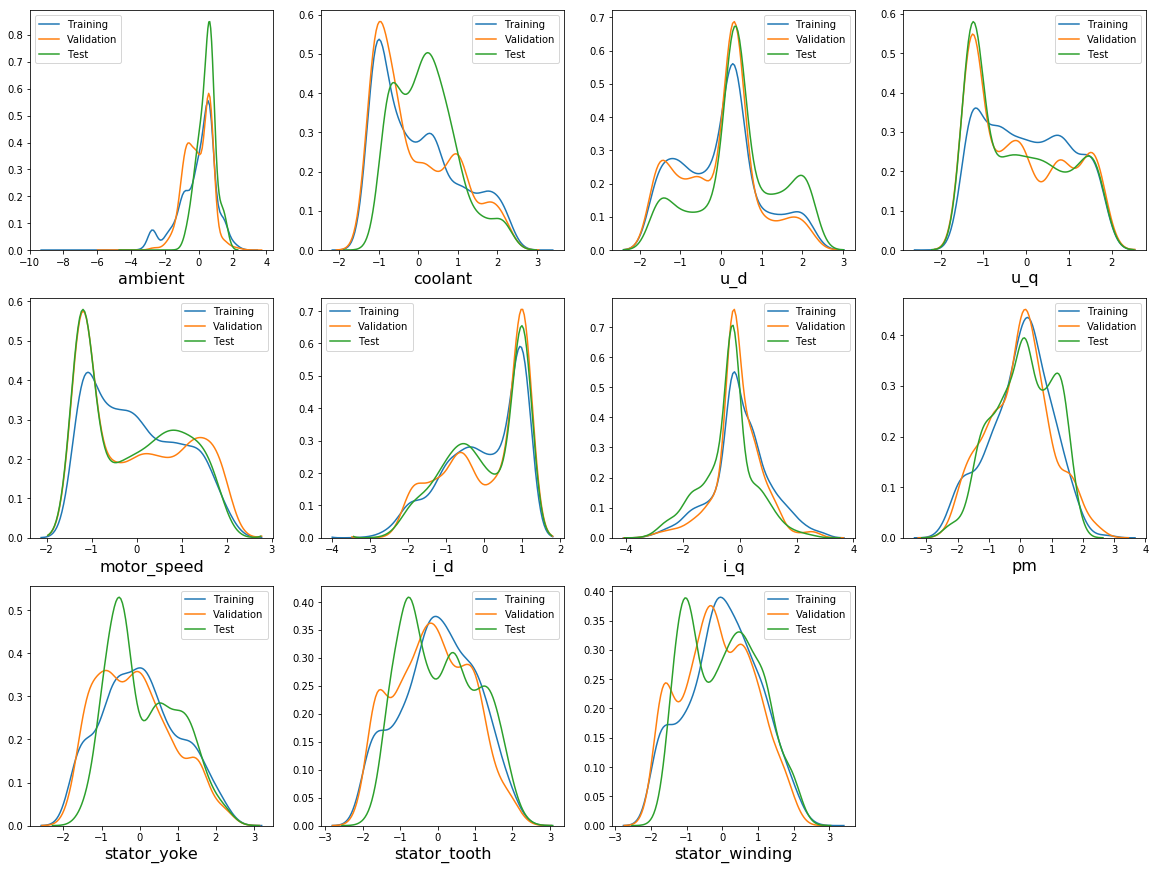
\includegraphics[width=\linewidth, height=10cm]{imgs/dist_plot.png}
    \caption{Distribution of the variables grouped by the division}
    \label{fig:dist_plot}
\end{figure}\\
In the Figure \ref{fig:corrplot} the correlation between the variables is shown. The target variables are highly correlated among themselves in particular the stator variables.
\begin{figure}[!h]
    \centering
    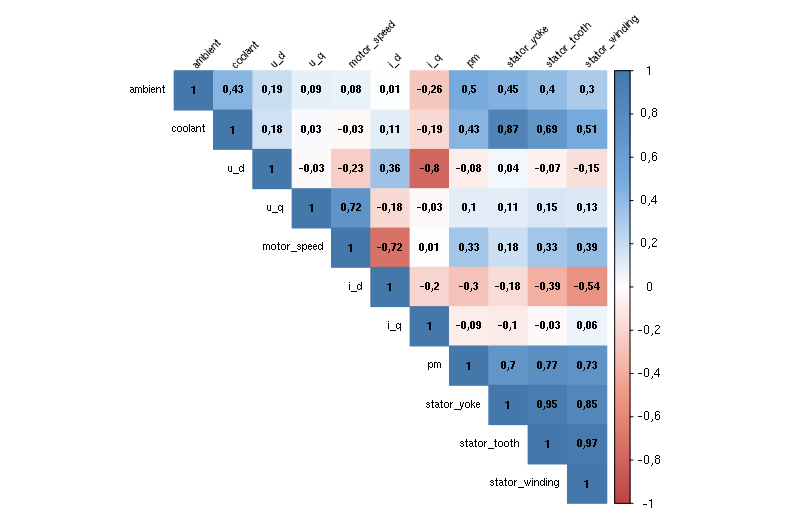
\includegraphics[width=10cm, height=10cm]{imgs/corrplot.png}
    \caption{Correlation Plot of the considered variables}
    \label{fig:corrplot}
\end{figure}\\
The data was already standardized but the variables doesn't have a normal distribution thus a normalization between 0 and 1 (using only the training set) is applied.

\section{The Methodological Approach}

This is the central and most important section of the report. Its objective must be to show, with linearity and clarity, the steps that have led to the definition of a decision model. The description of the working hypotheses, confirmed or denied, can be found in this section together with the description of the subsequent refining processes of the models. Comparisons between different models (e.g. heuristics vs. optimal models) in terms of quality of solutions, their explainability and execution times are welcome. 

%inifinitive generator!?
You should also mention any unforeseen problems you encountered when implementing the
system and how and to what extent you overcame them. Common problems are:
 difficulties involving existing software.


\section{Results and Evaluation}
The Results section is dedicated to presenting the actual results (i.e. measured and calculated quantities), not to discussing their meaning or interpretation. The results should be summarized using appropriate Tables and Figures (graphs or schematics). Every Figure and Table should have a legend that describes concisely what is contained or shown. Figure legends go below the figure, table legends above the table. Throughout the report, but especially in this section, pay attention to reporting numbers with an appropriate number of significant figures. 

\section{Discussion}
The discussion section aims at interpreting the results in light of the project's objectives. The most important goal of this section is to interpret the results so that the reader is informed of the insight or answers that the results provide. This section should also present an evaluation of the particular approach taken by the group. For example: Based on the results, how could the experimental procedure be improved? What additional, future work may be warranted? What recommendations can be drawn?


\section{Conclusions}
Conclusions should summarize the central points made in the Discussion section, reinforcing for the reader the value and implications of the work. If the results were not definitive, specific future work that may be needed can be (briefly) described. The conclusions should never contain ``surprises''. Therefore, any conclusions should be based on observations and data already discussed. It is considered extremely bad form to introduce new data in the conclusions.

\section*{References}

The references section should contain complete citations following standard form.  The references should be numbered and listed in the order they were cited in the body of the report. In the text of the report, a particular reference can be cited by using a numerical number in brackets as \cite{Lee2015} that corresponds to its number in the reference list. \LaTeX provides several styles to format the references

\bibliographystyle{IEEEtran}
\bibliography{references.bib}

\end{document}